\section{Introduction}
Iran is situated over Himalayan-Alpide seismic belt, which has frequently experienced strong shaking induced by earthquakes. The occurrence of these earthquakes has imposed notable destruction to the buildings and lifelines, and unfortunately, has caused extensive loss of human life. These earthquakes are categorized in various tectonic seismic zones. Different tectonic seismic regions have been defined for Iran in different studies.  Fig.~\ref{fig:Iran} shows the study region and different seismotectonic classification. Some of these studies defined more detailed division \citep{Nowroozi1976, Tavakoli1999}, and some of them defined one simplified province \citep{Stocklin1968, Takin1972, Berberian1976}. \citet{Mirzaei1998} divided Iran into five tectonic regions, including Azerbaijan-Alborz, Kopeh-Dagh, Zagros, Central-East Iran, and Makran. Regarding the other tectonic seismic regions, \citet{Karimiparidari2013} divided the Azerbaijan-Alborz tectonic seismic region into two regions, which are Azerbaijan and Alborz Mountain Range (hereinafter, Alborz). Azerbaijan, Alborz and Kopeh-Dagh tectonic seismic regions encompass most of northern Iran. Northern Iran has many highly populated cities (e.g., Tehran, Tabriz, and Mashhad), in which many destructive earthquakes have been reported.\\
\noindent
In northeastern of Iran, at least four historical earthquakes with $M>7$ struck in less than 200 years (1209, 1405) near the city of Neyshabur. Historical records show that in 1209, the district of Neyshabur from Neyshabur city in the west to Daneh village in the east was totally destroyed \citep{Berberian1999}.\\
\noindent
In the north western of Iran, a study of the seismic history of Tabriz based on available data shows that this region has been seismically active since 634 A.D. The historical earthquake data (pre 1900) illustrate that in earlier times the region was destroyed several times by major earthquakes. In 858, Tabriz was completely destroyed by a massive earthquake; the 1040 earthquake caused more than 50,000 causalities, and in 1936 due to the earthquake in Tabriz, most of the buildings fissured and even some collapsed \citep{Berberian1999}. Most recently, earthquakes with $M_w$ 6.1 in 1997 and $M_w$ 6.4 in 2012 occurred in Ardabil and Tabriz, respectively. These earthquakes caused around 1500 casualties and extensive damage \citep{USGS_ardabil,USGS_tabriz}.\\
\noindent
In north central Iran, in the Alborz region, a historical earthquake sequence occurred over a longer time period of 1100 years. At least three damaging historical earthquakes ruptured adjacent segments of the Mosha fault for a continuous distance of nearly 200 km: 958 A.D. (western segments), 1665 A.D. (eastern segments), and 1830 A.D. (central segments) \cite{Berberian1999}. Recently, the 1990 $M_w$ 7.4 Manjil-Rudbar earthquake caused extensive loss of life and significant damage \citep{USGS_manjil}. Based on existing documents, Tehran city and ancient Rey city have been destroyed completely several times by severe earthquakes with magnitudes greater than 7 \citep{Ambraseys2005}. \\
\noindent
Regarding historical earthquakes and the need for constructing new buildings and infrastructure, different seismic hazard analyses were conducted in Iran. Dividing Iran into 20 tectonic seismic regions, \citet{Tavakoli1999} prepared iso-acceleration contour lines and seismic hazard zonation for return periods of 75 and 475 years or 50\% and 10\% probability of exceedance in 50 years, based on major known lines and area source models. According to their study, North Tabriz fault zone and north of Tehran fault zone are in the highest acceleration contour. Maximum mean acceleration in the vicinity of these tectonic elements is predicted to be around 0.45 $g$ and 0.3 $g$ for a return period of 475 and 75 years, respectively. In the smaller scale, using the logic tree approach to compensate for uncertainties in the attenuation relationship, \citet{Ghodrati2003} presented a probabilistic seismic hazard assessment of metropolitan Tehran, the capital of Iran. The results showed that the PGA ranges from 0.27-0.46 $g$ for a return period of 475 years and from 0.33-0.55 $g$ for a return period of 950 years. In the last three decades, different seismic hazard analysis studies substantially improved the Iranian Code of Practice for Seismic Resistant Design of Buildings \citep{BHRC2014}. \citet{Ghodrati2013} conducted a seismic risk assessment for the city of Tehran using the Hazus method \citep{FEMA2003}. They represent that these efforts successfully decrease the total mean damage ratio in Tehran from 0.302739 in 1996 to 0.272859 in 2006.  Even though the results are satisfactory, the continuous improvement of procedures for defining the seismic hazard at regional (national) and local levels is essential for the optimum design of earthquake-resistant structures. In this study we use another model to overcome the aleatory and epistemic uncertainties regarding earthquake location and source mechanism in northern Iran.\\

In this study we used smoothed seismicity \citep{Frankel1995}. We divided northern Iran in three seismotectonic regions including Azerbaijan, Alborz, and Kopek Dagh. We also consider seismicity of part of Central-East Iran and Zagros regions. We computed seismic parameters and catalog completeness in these regions. Zagros and Central Iran seismotectonic regions have considerable effect on the Northern part. We used \citet{Karimiparidari2013} seismicity parameters in these regions.  We consider the $Mw5$ earthquake as a threshold magnitude  for structural damage. In order to consider damage to the historical masonry building we also considered $Mw4.5$ as a threshold for structural damage to these kind of building. 


\begin{figure} [H]
\centering
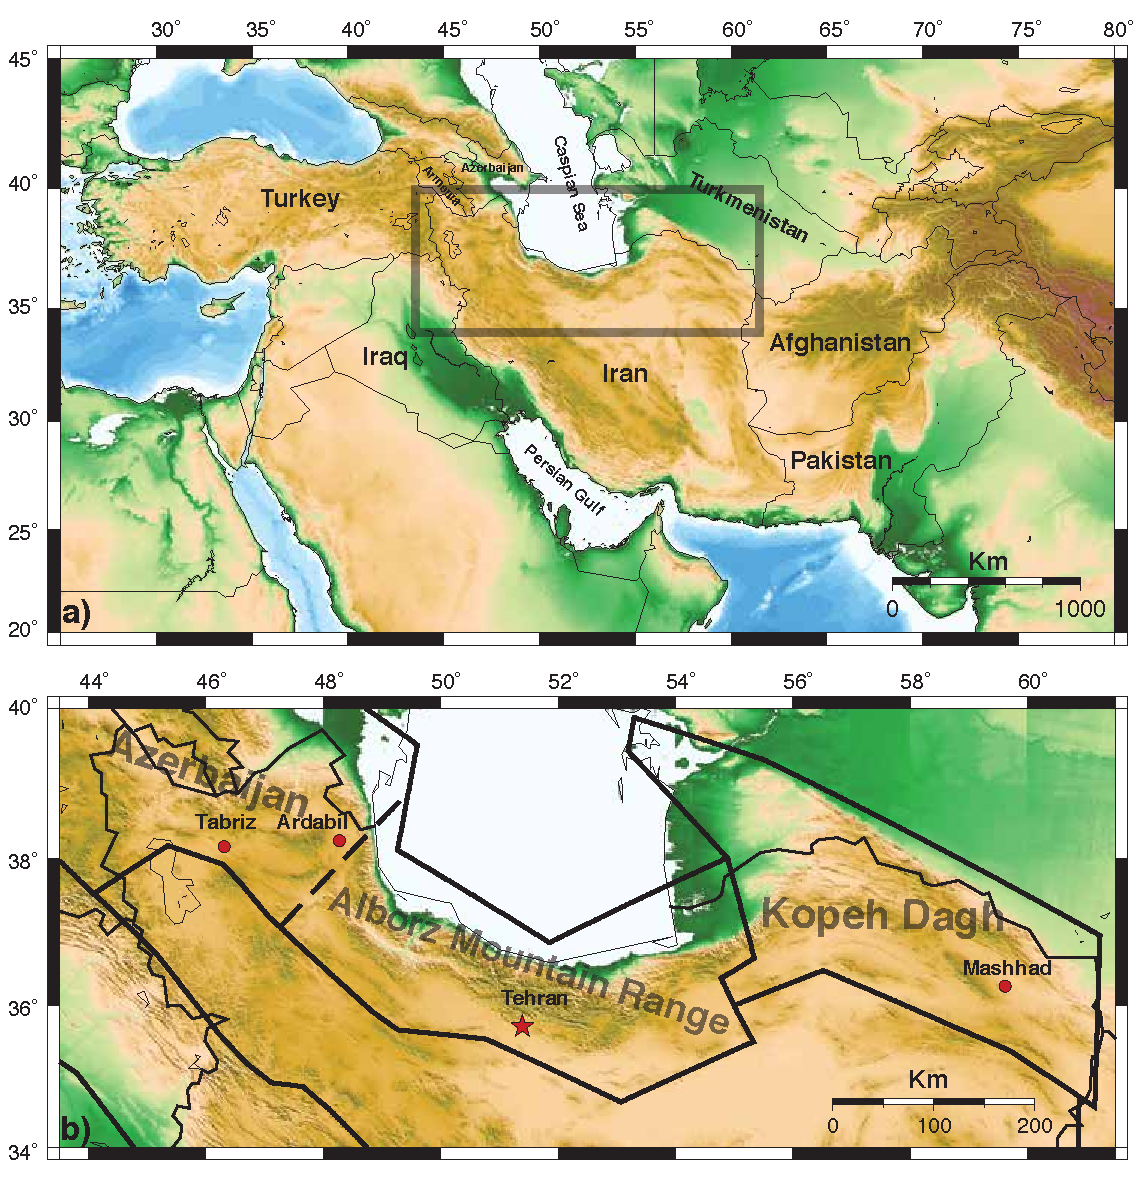
\includegraphics[scale=0.7]{figures/pdf/Figure1.pdf} 
\caption{ a) Map of Iran and surrounding countries. The study area is presented in gray box. b) The study area containing seismotectonic provinces after \citet{Mirzaei1998}, and location of big cities. Dashed line is the subdivision that is proposed by \citet{Karimiparidari2013}. }
 
\label{fig:Iran}
\end{figure}





\noindent
Recently, northern Iran has been studied in detail from different seismological points of view. \citet{Nemati2015} studied the most recent 200 years' seismicity in northern Iran. The frequency of shocks vary widely from one mainshock per 6 years (0.17 event/ year) for the Azerbaijan region to 13 earthquakes per 4 years for the Kopeh-Dagh (3.25 event/year) region. Recorded events and a partially quiet period suggest that strong earthquakes must be expected in Alborz within the next decade, which may cause significant damage to northern Iran. Using newly recorded data, \citet{Zafarani2014} defined the most appropriate attenuation relationship for use in the Azerbaijan, Alborz and Kopeh-Dagh regions. In this study we use an updated catalog from International Institute of Earthquake Engineering and Seismology \citep{IIEES} and the recently confirmed attenuation relationship for northern Iran \citep[i.e.,][]{Kalkan2004} in order to conduct seismic hazard analysis from background seismicity. We follow \citet{Frankel1995} approach to calculate hazard from background seismicity for northern Iran. This differs from the traditional approach in which area source zones are drawn around seismicity or tectonic provinces for the calculation of seismic hazard \citep{Cornell1968}. \\
\noindent
Having limited knowledge in seismic sources, \citet{Frankel1995} used this approach to map seismic hazards in central and eastern United States. The major features of Frankel's approach are to abandon tectonic seismic zones and to use point sources in seismic hazard analysis. This method is simpler for hazards calculation and is based solely on recorded seismicity history. In the smoothed-seismicity approach we avoid choosing zone boundaries that are sometimes poorly delineated by data and drawn by subjectively merging geological and seismological information. Even though probabilistic seismic hazard involving fault sources is more realistic and accurate, recognizing sources could present considerable uncertainty. \citet{Masson2006} studied 19 points of the GPS network that have been installed in the framework of French-Iranian cooperation. At some stations (e.g., the ATTA station) they expect to record significant movement, based on the region's historical activity.  Surprisingly, they recorded velocity of $0\  mm/yr$. \\
\noindent
The smoothed-seismicity method simply assumes that patterns of historical earthquakes predict future activity. Using background seismicity, \citet{Cao1996} conducted a seismic hazard estimation study in southern California. They concluded that one could obtain similar results implementing background seismicity to those obtained by introducing zones for areas with well-recorded seismicity patterns. \citet{Lapajne1997} used spatially smoothed seismicity modeling to acquire a seismic hazard outlook in Slovenia. They defined 4 different models with different correlation distances, including a model based of the total released seismic energy. They gained an acceptable PGA in comparison with other seismic hazard approaches. \citet{Akinci2004} estimate the seismic hazard in central and northern Italy using smoothed historical seismicity. Their results showed that the smoothed seismicity approach gives reasonable regionalized results without introducing seismogenic zones. This approach has also been used in many regions with different seismicity patterns \citep{Wesson1999, Klein2001, Hamdache2008, Kalkan2009, Moschetti2014, Boyd2008}. We generate maps of peak ground acceleration with 2\% and 10\% probabilities in exceedance of 50 years in northern tectonic seismic zones, including Azerbaijan, Alborz, and Kopeh-Dagh and in central-eastern Iran and a small portion of the northern Zagros region. Since we do not introduce faults into the model, our results show variability due only to the characteristics of seismicity and ground motion. 



\section{Seismic regions and seismicity rate}
With respect to different seismicity rates of the regions \cite{Nemati2015}, as well as the completeness of the seismic catalog, the study region is divided into three zones. Each of these zones is characterized by its respective seismicity parameters values, including b-value and maximum magnitude ($M{_{max}}$). A review of Iran's historical earthquakes (pre 1900) is provided by \citet{Ambraseys2005}. \citet{Karimiparidari2013} converted all historical earthquakes to a unified magnitude ($M_w$), which we use as a historical catalog. The International Institute of Earthquake Engineering and Seismology of Iran \citep{IIEES} has reported the instrumental data, which also involves earthquakes from border countries which have considerable affect in the seismicity of Iran's border cities. 
In the present study, historical data are integrated with instrumental data. We use the tectonic seismic division to categorized the data according to the seismic tectonic regions. 
\subsection{Alborz Mountain Range (Alborz)}
Tehran region has active reverse faults, which are parallel to the northwest-trending structural gain of the Alborz Mountains belt. Here a series of historical earthquakes occurred within a time period of more than 1100 years. Four earthquakes with magnitude more than 7 devastated the Tehran region in four centuries period, from 743 to 1177, but in the last 800 years, only one earthquake at 1830 has struck this region. At least three damaging earthquakes in 958 (western segments), 1655 (eastern segments), and 1830 (central segments), ruptured adjacent segments of the Mosha fault, located in northern Tehran.
The North Tehran Thrust (NTT) adds more complexity due to the presence of south-dipping reverse faults, which are in part blind, such as the Davudieh, Shian, and Bagh-E Feyz.
The northwest continuation of the Alborz Mountains, known as the Rocks of the Talesh Mountains, have been thrust northeastward and eastward over rocks of the south Caspian depression. An earthquake with Ms 6.0 in 1978 led to a focal mechanism consistent with a low-angle thrust \citep{Berberian1999}.



\subsection{Azerbaijan}
There were three earthquakes from 1721-86 that ruptured the North Tabriz Fault system from southeast to northwest. The Tabriz region is in the Araxes structural block of northwestern Iran, southwest of the continuation of the western Alborz Mountains towards the Caucasus. The North Tabriz Fault (NTF) is a complex northwest-trending structure, which contains evidence observed on aerial photographs, and vertical displacement with the north side up, of right-lateral strike-slip displacement \citep{Berberian1999}.
The NTF system and nearby reverse faults ruptured from southeast to northwest in three earthquakes over 65 years: the Shebli earthquake with magnitude 7.3 in 1721 on the southeastern NTF with a surface rupture more than 35 km long, reported by \citet{Jones1834} the Tabriz earthquake with magnitude 7.4 in 1780 on the northwestern NTF, with a surface rupture more than 42 km long and vertical separation of 2 to 4 $m$; and the Marand-Mishu earthquake with magnitude of 6.3 in 1786 on the Mishu reverse fault and the Sufian segment of the NTF. Another earthquake with  magnitude 5.5 struck the Tasuj reverse fault farther west in 1807 and an earthquake of M 6.7 took place along the South Bozqush reverse fault farther southeast in 1879. Prior to the 1721-86 earthquake sequence, Tabriz was shaken by earthquakes in 858 (M 6.0), 1042 (M 7.3), 1273 (M ~ 6.5), and 1304 (M 6.7)\citep{Berberian1999}. 


\subsection{Kopeh Dagh}
The main Kopeh-Dagh fault system has experienced some historic earthquakes. Ashgabat, the capital city of Turkmenistan, was destroyed by an earthquake of Ms 7.2 in 1948 and destroyed more than 30 villages in Iran. This was the strongest earthquake to strike this region since at least 1455.
The main Kopeh-Dagh fault consists of several partly overlapping segments parallel to the overall $NW - SE$ structure with step-overs. The regions of overlap are characterized by shorter south-dipping thrust faults striking about $E - W$ \citep{Berberian2001}. \citet{Trifonov1978} reported active displacement along the main Kopeh-Dagh fault for more than 500 km. 
Massive destruction of the capital city of Mithradatkert is attributed to the 10 BC event Ms 7.1, roughly 30 kilometers from the border of Iran (Nesa mound) \citep{Berberian2001}.
The Neyshabur sequence of four earthquakes between 1209 and 1405 respected the segment boundary between the Neyshabur and Binalud reverse fault system \citep{Berberian1999}.


